 \documentclass[column,amsmath,amssymb,floatfix]{revtex4}

% ---- Pacotes para formatação de texto e símbolos matemáticos ----
\usepackage{amsmath}
\usepackage{amssymb}
\usepackage{amsfonts}

% ---- Pacotes para gráficos e tabelas ----
\usepackage{graphicx}
\usepackage{dcolumn}
\usepackage{float}

% ---- Pacotes para formatação e personalização de cores e fontes ----
\usepackage{xcolor}
\usepackage{color}
\usepackage{bm}
\usepackage{titlesec}

% ---- Pacotes para código fonte ----
\usepackage{listings}
\usepackage{verbatim}

\lstdefinestyle{customc}{
  belowcaptionskip=1\baselineskip,
  breaklines=true,
  frame=none,
  xleftmargin=\parindent,
  language=python,
  showstringspaces=false,
  basicstyle=\footnotesize\ttfamily,
  keywordstyle=\bfseries\color{green!40!black},
  commentstyle=\itshape\color{purple!40!black},
  identifierstyle=\color{blue},
  stringstyle=\color{orange},
}

\lstdefinestyle{customasm}{
  belowcaptionskip=1\baselineskip,
  frame=trBL,
  xleftmargin=\parindent,
  language=[x86masm]Assembler,
  basicstyle=\footnotesize\ttfamily,
  commentstyle=\itshape\color{purple!40!black},
}

\lstset{escapechar=@,style=customc}

% ---- Pacotes de idioma e codificação ----
\usepackage[brazilian]{babel}
\usepackage[utf8]{inputenc}
\usepackage[T1]{fontenc}

% ---- Pacote para criação de links e hiperlinks ----
\usepackage{hyperref}

% ---- Definição de comandos personalizados ----
\newcommand{\PAR}[1]{\left({[#1]}\right)}

% ---- Ajustes de espaçamento para títulos ----
\titlespacing\section{0pt}{12pt plus 4pt minus 2pt}{8pt plus 2pt minus 2pt}
\titlespacing\subsection{0pt}{12pt plus 4pt minus 2pt}{8pt plus 2pt minus 2pt}
\titlespacing\subsubsection{0pt}{12pt plus 4pt minus 2pt}{0pt plus 2pt minus 2pt}

\begin{document}

\title{Estudo do Problema de Dirichlet para a Equação de Poisson com Discretização Finita}
\author{Julio Cezar de Moura Lima \\ Lucas Amaral Taylor}

\begin{abstract}
    \baselineskip 11pt
    \begin{center}
        Este relatório trata do problema de Dirichlet para a equação de Poisson, que é discretizado em um quadrado unitário utilizando o método de diferenças finitas com espaçamento $h = \frac{1}{N}$. As equações que descrevem $U_{mn}$, juntamente com as condições de contorno, são organizadas em um sistema linear. Esse sistema é então resolvido utilizando uma ordenação lexicográfica para facilitar o processo de solução numérica.
    \end{center}
\end{abstract}


\maketitle

    \section{Introdução}
        Este relatório aborda a solução numérica da equação de Poisson no domínio unitário $\Omega = (0,1) \times (0,1)$ com condições de contorno de Dirichlet. A equação a ser resolvida é:
        \begin{equation*}
             -\Delta u(x, y) = f(x, y), \quad (x, y) \in \Omega, 
        \end{equation*}
    
        com as condições de fronteira:
        \begin{equation*}
            u(\xi, \eta) = g(\xi, \eta), \quad (\xi, \eta) \in \partial\Omega.
        \end{equation*}
        
        Utilizamos o método de diferenças finitas centradas para discretizar a equação, transformando-a em um sistema linear. A discretização do domínio em uma malha de tamanho $N \times N$, com espaçamento $h = \frac{1}{N}$, resulta na seguinte equação:
        \begin{equation*}
            \frac{1}{h^2}(-U_{m-1,n} - U_{m,n-1} + 4U_{mn} - U_{m,n+1} - U_{m+1,n}) = f_{mn}, \quad 1 \leq m,n \leq N-1.
        \end{equation*}
    
        Esse sistema é resolvido usando bibliotecas como \texttt{numpy} e \texttt{scipy}. Simulações foram realizadas para diferentes $N$ e comparadas com soluções exatas. Os resultados demonstram a eficiência do método, com erros decrescendo à medida que $N$ aumenta. 
    
    \section{Fundamentos teóricos}
        Na presente seção discutiremos os principais aspectos teóricos, discutidos em aula, que envolvem o processo de discretização da equação de Poisson no domínio em questão, são elas: o problema do contorno e a estimação do erro.
        
        O problema do contorno é fundamental, visto que são restrições impostas na fronteira do domínio que influenciam diretamente as soluções da equação diferencial dentro desse domínio. 

        Além disso, abordaremos a respeito da estimação do erro, discorrendo sobre a convergência dele e sua consistência, a fim de mostrar a eficiência do método empregado. 
        
        As principais referências utilizadas para redigir esta seção estão presentes em \cite{Chen2014} e \cite{Butler2021}, onde poderão ser encontradas as devidas demonstrações e demais detalhes dos fatos apresentados. Por fim, os tópicos foram selecionado com base na metodologia empregadas em aula \cite{Kuhl2024}. 
    
        \subsection{Problema de contorno}

            No que diz respeito a \textit{problema do contorno}, abordaremos sobre a \textit{condição de Dirichlet} e a \textit{condição de Neumann}. Para a condição de Dirichlet, temos a equação de Poisson:
            \begin{equation*}
                -\Delta u = f \quad \text{em} \, \Omega,
            \end{equation*}
            com a condição de contorno prescrita:
            \begin{equation*}
                u = g \quad \text{em} \, \partial \Omega,
            \end{equation*}
            
            Nesse caso, o valor da função $u$ é fixado na fronteira pela condição $u = g$. No método de diferenças finitas, isso significa que as incógnitas associadas aos nós na fronteira são eliminadas do sistema linear, substituídas pelos valores prescritos de $g$. A matriz do sistema linear resultante é modificada para refletir essa eliminação, o que pode ser feito de diferentes formas. Uma abordagem comum é ajustar diretamente os valores no vetor de solução.
            
            Já para a condição de Neumann, temos a equação de Poisson:
            \begin{equation*}
                -\Delta u = f \quad \text{em} \, \Omega,
            \end{equation*}
            com a condição de contorno:
            \begin{equation*}
                \frac{\partial u}{\partial n} = g \quad \text{em} \, \partial \Omega,
            \end{equation*}
            onde $\frac{\partial u}{\partial n}$ é a derivada normal de $u$ na fronteira $\partial \Omega$. Essa condição especifica o fluxo na direção normal à fronteira, em vez de fixar diretamente os valores de $u$.
            
            No método de diferenças finitas, essa derivada normal pode ser aproximada usando diferenças finitas. Para melhorar a precisão, introduzem-se pontos fantasmas fora do domínio $\Omega$. Por exemplo, uma aproximação de primeira ordem para a derivada normal em $x = x_1$ é:
            \begin{equation*}
                \frac{\partial u}{\partial n} \approx \frac{u_1 - u_2}{h} + \mathcal{O}(h),
            \end{equation*}
            onde $h$ é o espaçamento da malha. Para uma aproximação de segunda ordem, pode-se usar:
            \begin{equation*}
                \frac{\partial u}{\partial n} \approx \frac{u_0 - u_2}{2h} + \mathcal{O}(h^2),
            \end{equation*}
            onde $u_0$ é o valor no ponto fantasma fora do domínio.
            
            Para eliminar o ponto fantasma da equação, utiliza-se a condição de contorno de Neumann e manipula-se o sistema de equações de forma a manter a simetria da matriz. Por exemplo, para um ponto $(x_1, y_j)$, a equação é ajustada para:
            \begin{equation*}
                2u_{1,j} - u_{2,j} - 0.5u_{1,j+1} - 0.5u_{1,j-1} = 0.5h^2 f_{1,j} + h g_{1,j}.
            \end{equation*}
            Isso garante que a condição de Neumann seja satisfeita com precisão.
            
            A condição de Neumann requer que as funções $f$ e $g$ satisfaçam a condição de compatibilidade:
            \begin{equation*}
                -\int_\Omega f \, dx = \int_{\partial \Omega} g \, dS,
            \end{equation*}
            que garante a consistência entre o fluxo total na fronteira e a integral da fonte $f$ sobre o domínio $\Omega$. Se essa condição não for satisfeita, a equação pode não ter solução. No contexto de diferenças finitas, essa compatibilidade é garantida ao ajustar o termo constante na equação, como em:
            \begin{equation*}
                \sum_{i=1}^{N} f_i = 0,
            \end{equation*}
            onde $f_i$ são os valores discretos da função $f$ nos nós da malha. Detalhes e demonstrações em \cite{Chen2014} e \cite{Butler2021}.

        
        \subsection{Análise do Erro}
                Primeiramente, é importante destacar que analisamos o erro partindo da metodologia apresentada em sala \cite{Kuhl2024} e detalhamento proveniente de \cite{Chen2014}.
                
            \subsubsection{Consistência}
                Definiremos duas variáveis:
                \begin{align*}
                    U_{mn} &: \text{ Solução do problema discreto}\\
                    u_{mn} &: \text{ Valor da solução do problema contínuo em $(x_n, y_n)$}
                \end{align*}
    
                A partir do processo de discretização, temos que:
                \begin{align*}
                    \frac{u_{m, n-1} + u_{m+1, n} - 4u_{m, n} + u_{m+1, n} + u{m, n+1}}{h^2} &= f_{m,n} + d_{m,n}\\
                    \frac{U_{m, n-1} + U_{m+1, n} - 4U_{m, n} + U_{m+1, n} + U{m, n+1}}{h^2} &= f_{m,n}
                \end{align*}
    
                O erro pode ser expresso como a diferença entre $u_{m,n}$ e $U_{m,n}$, isto é:
                \begin{equation*}
                    E_{m,n} = u_{m,n} - U_{m,n}
                \end{equation*}
    
                Assim, 
                \begin{equation*}
                    \frac{E_{m, n-1} + E_{m+1, n} - 4E_{m, n} + E_{m+1, n} + E{m, n+1}}{h^2} = d_{m,n}, \quad 1 \leq m, n \leq N
                \end{equation*}
    
                Com
                \begin{equation*}
                    E_{0,m} = E_{N+1, n} = E_{m, 0} = E_{m, N+1} = 0
                \end{equation*}
    
                Ou seja, o operador de diferenças finitas aplicado ao erro $E_{m,n}$ pode ser expresso por: 
                \begin{equation*}
                    \left(\Delta_h E \right)_{m,n} = d_{m, n}, \quad 1 \leq m, n \leq N 
                \end{equation*}
    
                Como discutido em \cite{Chen2014}, o termo $d_{mn}$ representa o erro de truncamento, que surge ao aproximar o operador contínuo $\Delta$ pelo operador de diferenças finitas $\Delta_h$. Para métodos de diferenças finitas de segunda ordem, o erro de truncamento é proporcional a $h^2$, resultando na seguinte aproximação:
                \begin{equation*}
                    \Delta_h u_{mn} = \Delta u_{mn} + \mathcal{O}(h^2),
                \end{equation*}
                
                onde $\mathcal{O}(h^2)$ é o erro associado à discretização. Assim, o erro residual $d_{mn}$ é estimado como:
                \begin{equation*}
                    d_{mn} \leq C_4 \cdot h^2,
                \end{equation*}
                
                com $C_4$ dependendo da regularidade de $u$ (supondo que $u \in C^4$). Essa estimativa reflete a consistência do método, com o erro diminuindo à medida que $h$ se refina.
            
            \subsubsection{Estimação do erro}
                Primeiro, enunciaremos o \textit{Princípio do Máximo (mínimo)}, cuja a demonstração estará omitida, mas apresentada devidamente em \cite{Chen2014}.
                    
                Se  $(\Delta_h v)_{mn} \geq 0 \ (\leq 0), 1 \leq m, n \leq N$, então o máximo (mínimo) de $v$ é atingido na fronteira $\Gamma_h$:
                \begin{align*}
                    \max v &= \max_{\Omega_h} v = \max_{\Gamma_h} v\\
                    \min v &= \min_{\Omega_h} v = \min_{\Gamma_h} v
                \end{align*}
        
                A enunciação do \textit{Princípio do Máximo (mínimo)} é fundamental, pois ele implica que a solução numérica obtida no interior do domínio está limitada pelos valores na fronteira, o que auxilia na estimação do erro. Isto posto, podemos abordar sobre a estimação do erro. 
                
                No método de diferenças finitas, a solução numérica $V_{mn}$ para a equação $(\Delta_h V)_{mn} = F_{mn}$ com condições de contorno de Dirichlet $V = 0$ na fronteira $\Gamma_h$ pode ser controlada pela função forçante $F_{mn}$.

                Aplicando o \textit{Princípio do Máximo}, concluímos que o erro no interior do domínio é limitado pelo valor máximo de $F_{mn}$:

                \begin{equation*}
                    |V_{mn}| \leq \frac{1}{8} \max_{1 \leq m,n \leq N} |F_{mn}|.
                \end{equation*}

                Isso garante que o erro numérico dentro do domínio não cresce além de uma fração do valor máximo de $F_{mn}$.
                
                Além disso, ao considerar a função auxiliar $W(x, y)$, cuja derivada discreta $\Delta_h W_{mn} = 1$, ajustamos a estimativa de erro para obter:
                \begin{equation*}
                    \Delta_h v_{mn} + \|F\|_\infty W_{mn} \geq 0,
                \end{equation*}
                
                onde $\|F\|_\infty$ é a \textbf{norma do máximo} de $F$, definida como:
                \begin{equation*}
                    \|F\|_\infty = \max_{1 \leq m,n \leq N} |F_{mn}|,
                \end{equation*}
                isto é, o maior valor absoluto de $F_{mn}$ no domínio discretizado.
                
                Isso confirma que o erro $v_{mn}$ é limitado por $\|F\|_\infty$, reforçando a estabilidade do método. Demonstração em \cite{Kuhl2024}.
                
    \section{Implementação e explicação da resolução da tarefa}

        Para explicação das tarefas desempenhadas no trabalho, vamos iniciar com o exercício de número 1.
                    
        O problema se inicia obtendo $f$ em ambos os casos em que $u_{exata}$ é definida.Utilizando a definição bastaria que fosse atribuído $-\Delta u$ para achar cada $f$. 

        \begin{lstlisting}
        # funcao u (item a)
        u = lambda x, y: x**4 - 6*x**2*y**2 + y**4
        f_u = lambda x, y: -12*(x**2 + y**2)
        
        # Funcao v (item b)
        v = lambda x, y: np.exp(x) * np.sin(y)
        f_v = lambda x, y: 0
        \end{lstlisting}

        
        Em seguida realizamos a construção de uma função que estabelece $A$ e $b$, no que tange, a resolução do problema $AU = b$. Note que a mesma será usada essencialmente em ambos os exercícios.

        \begin{lstlisting}
        def poisson_system(N: int, f: float, g: float):
        h = 1/N
        n = (N-1)**2 # numero de variaveis presentes no sistema
        diagonals = [-1, -1, 4, -1, -1] # valores que serao atribuidos as diagonais de A
        offsets = [-N+1, -1, 0, 1, N-1] # confere o deslocamento das diagonais
        
        # matriz A iniciada
        A: csc_array = diags(diagonals=diagonals, offsets=offsets, shape=(n,n)).tocsc()
        
        # vetor b (termos da equacao e cond. de contorno)
        b = np.zeros(n)
        
        # Preenchimento de b com f (pontos internos)
        for k in range(1, N):
            for j in range(1, N):
                i = (k - 1) * (N-1) + (j-1) # indice lexicografico
                x, y = k * h, j * h
                b[i] = h ** 2 * f(x, y)
        
        # Bordas (esq -> dir) & (inf -> sup): cond. de contorno
                if k == 1:
                    b[i] -= g(0, y)  # borda esquerda
                if k == N - 1:
                    b[i] -= g(1, y)  # borda direita
                if j == 1:
                    b[i] -= g(x, 0)  # borda inferior
                if j == N - 1:
                    b[i] -= g(x, 1)  # borda superior
        
        return A, b
        \end{lstlisting}
        
        Tendo esta implementação, vamos partir para finalização, determinando $g$ e solucionando o sistema, de modo que teremos a solução numérica e, portanto, possibilidades de visualizá-la graficamente.
        
        \begin{lstlisting}
        g = lambda x,y: exact(x,y) # atribui  u_exata no caso solicitado
        
        A, b = poisson_system(N, f, g) #(i)
        numeric = linalg.spsolve(A,b)  #(ii)
        plot_solution(N, exact, numeric, title) #(iii)   
        \end{lstlisting}

        Tendo solucionado o problema 1, para o problema 2 partiremos dos mesmos princípios já introduzidos.
        
        \begin{lstlisting}
        # Iniciando as funcoes do problema
        u = lambda x,y: np.cos(x) * np.sin(y)
        f = lambda x,y: -2 * np.cos(x) * np.sin(y)
        \end{lstlisting}

        Vamos partir da análise de funções que serão usadas na resolução dos itens (b) e (c). O sistema que retorna $A$ e $b$ segue o mesmo que foi mencionado para o exercício 1. Desse modo para avaliarmos o erro, faremos uso da seguinte função:
        
        \begin{lstlisting}
        def error_function(N, exact, numeric) -> pd.DataFrame:
            x = np.linspace(0, 1, N+1)
            y = np.linspace(0, 1, N+1)
            X, Y = np.meshgrid(x, y)
        
            # solucao exata nos pontos da grade
            U_exata = exact(X, Y)
        
            # Inserir solucao numerica nos pontos internos
            U_numerica = np.zeros((N+1, N+1))
            U_numerica[1:N, 1:N] = numeric.reshape((N-1, N-1))
        
            # Calcular o erro absoluto
            errors = np.abs(U_exata - U_numerica) # Erro em modulo
        
            # Dataframe em pandas para armazenar os erros (row, column) = (X_i, y_i)
            df = pd.DataFrame(errors, 
                              columns=[f"Erro y={i/(N+1):.2f}" for i in range(N+1)],
                              index=[f"x={i/(N+1):.2f}" for i in range(N+1)])
            return df   
        \end{lstlisting}
        
        Portanto, com a coletânea de funções necessárias basta resolver o sistema, calcular o erro relativo à $u_{exata}$ e assim plotar simulações em cada $N$.
        
        \begin{lstlisting}
        def solve_system(N, f, u):
            g = lambda x,y: u(x,y)
        
            A, b = poisson_system(N, f, g)        #(i)
            numeric = linalg.spsolve(A,b)         #(ii)
            plot_solutions(N, u, numeric)         #(iii)
            print(error_function(N, u, numeric))  #(iv)
        
        print("Simulacoes")
        for N in [50, 100, 200]:
            print(f"N = {N}")
            solve_system(N, f, u)
        \end{lstlisting}
        
    \section{Apresentação dos resultados}
        \begin{enumerate}
            \item Construir os exemplos a partir da função dada(obtenha $f$ e $g$) a partir da solução $u$, implemente esses exemplos e realize simulações para $N = 20, 50$ e $100$:
            \begin{enumerate}
                \item $u(x,y) = x^4 - 6x^2y^2 + y^4$.

                \textbf{Solução:}

                \begin{figure}[H]
                    \centering
                    \begin{minipage}{0.32\textwidth}
                        \centering
                        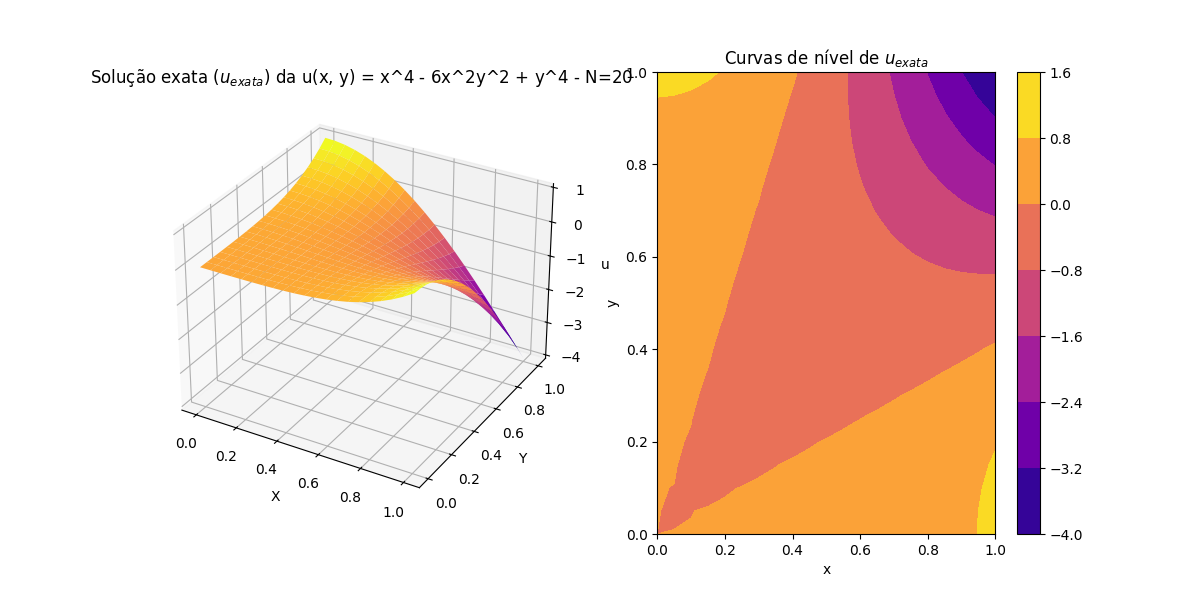
\includegraphics[width=\textwidth]{TAREFA_01/img/Problem1/a_20.png}
                        \caption{Simulação 1A com $N = 20$}
                    \end{minipage}
                    \hfill
                    \begin{minipage}{0.32\textwidth}
                        \centering
                        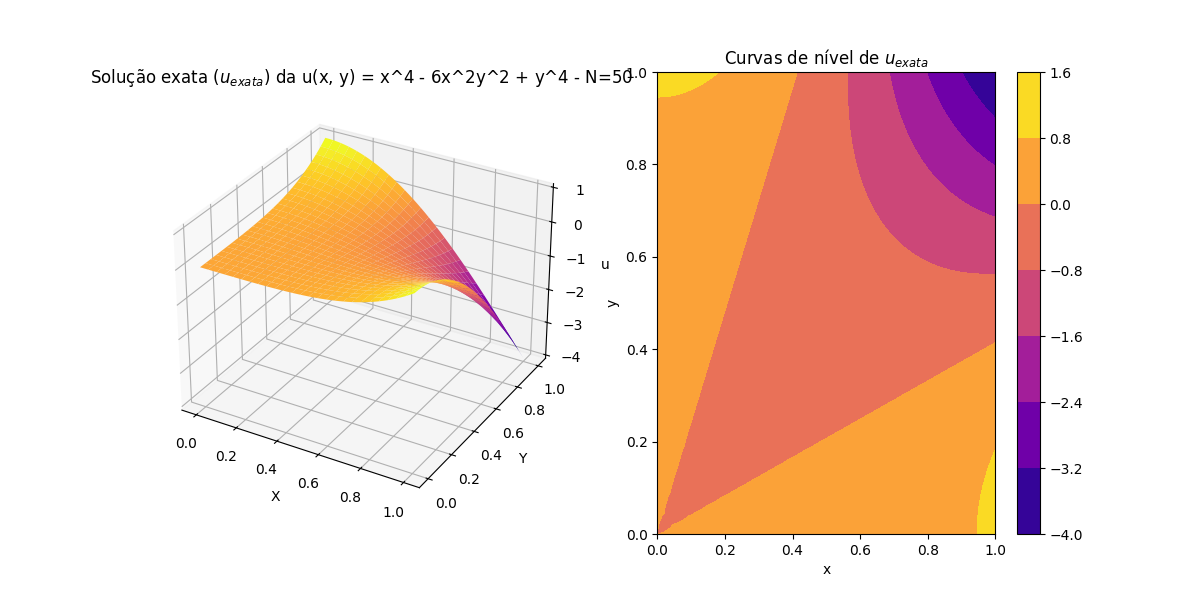
\includegraphics[width=\textwidth]{TAREFA_01/img/Problem1/a_50.png}
                        \caption{Simulação 1A com $N = 50$}
                    \end{minipage}
                    \hfill
                    \begin{minipage}{0.32\textwidth}
                        \centering
                        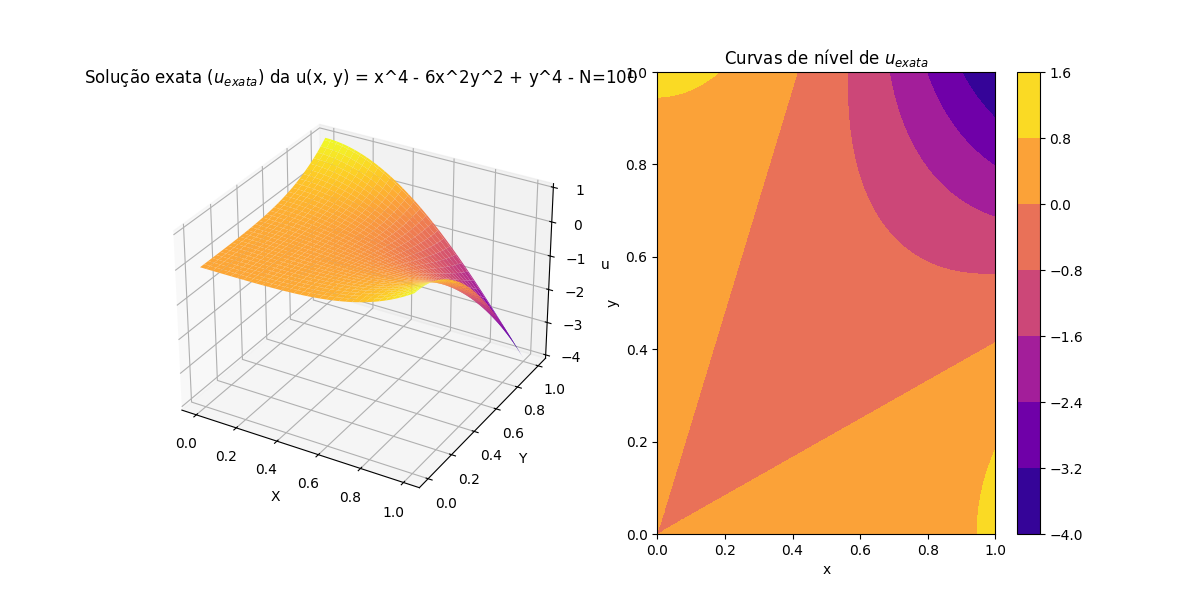
\includegraphics[width=\textwidth]{TAREFA_01/img/Problem1/a_100.png}
                        \caption{Simulação 1A com $N = 100$}
                    \end{minipage}
                \end{figure}
            
                \item $u(x,y) = e^x \sin(y)$

                \textbf{Solução:}
                
                \begin{figure}[H]
                    \centering
                    \begin{minipage}{0.32\textwidth}
                        \centering
                        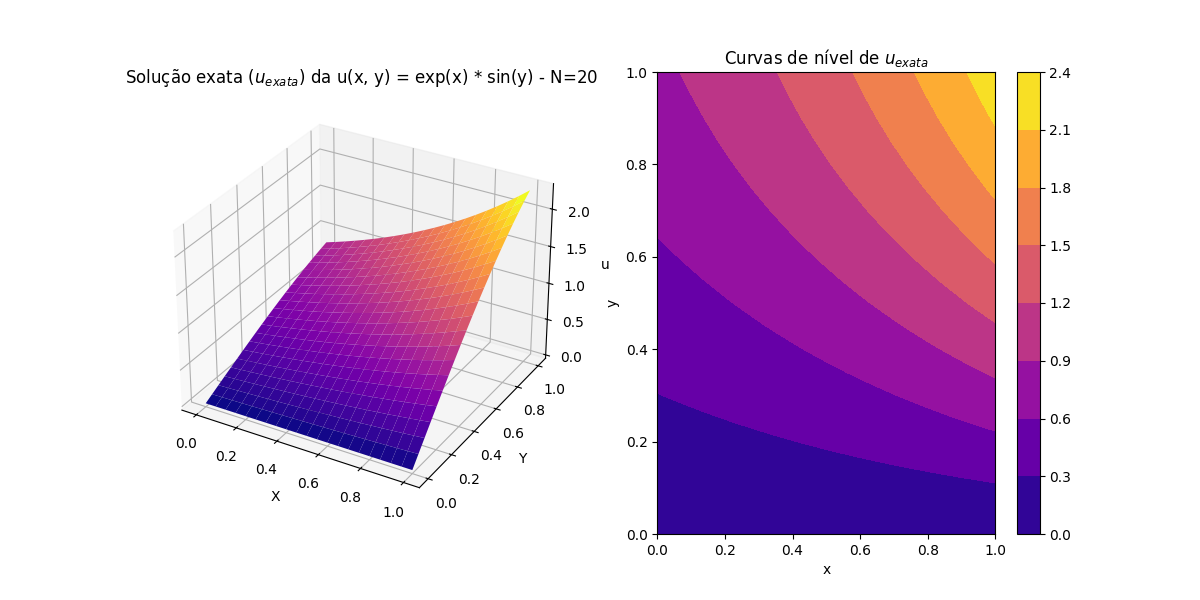
\includegraphics[width=\textwidth]{TAREFA_01/img/Problem1/b_20.png}
                        \caption{Simulação 1B com $N = 20$}
                    \end{minipage}
                    \hfill
                    \begin{minipage}{0.32\textwidth}
                        \centering
                        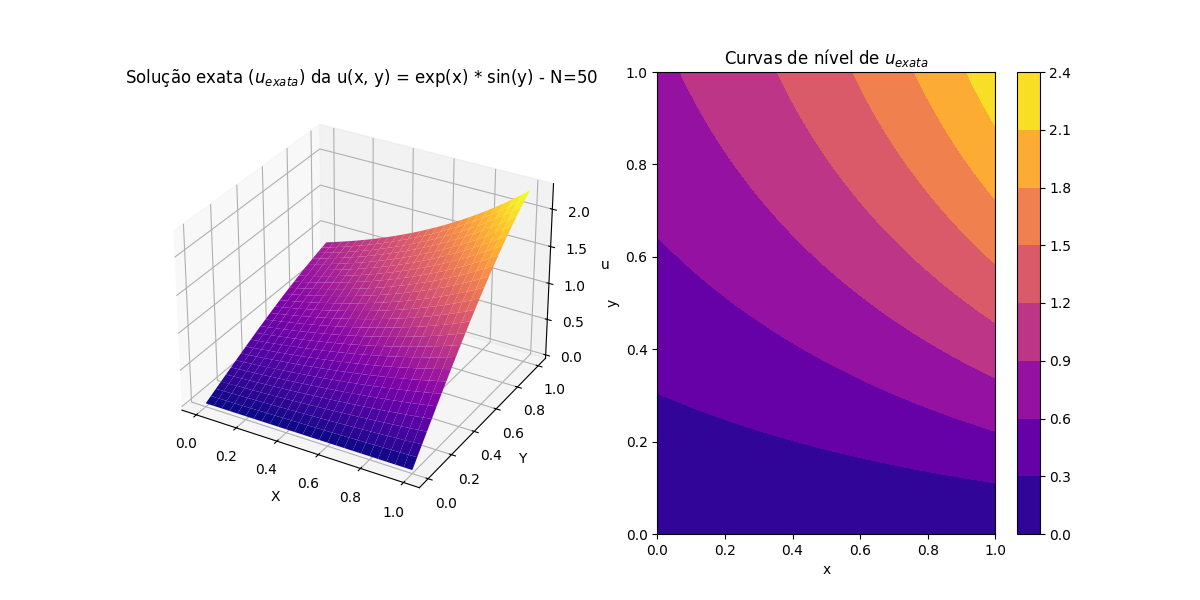
\includegraphics[width=\textwidth]{TAREFA_01/img/Problem1/b_50.png}
                        \caption{Simulação 1B com $N = 50$}
                    \end{minipage}
                    \hfill
                    \begin{minipage}{0.32\textwidth}
                        \centering
                        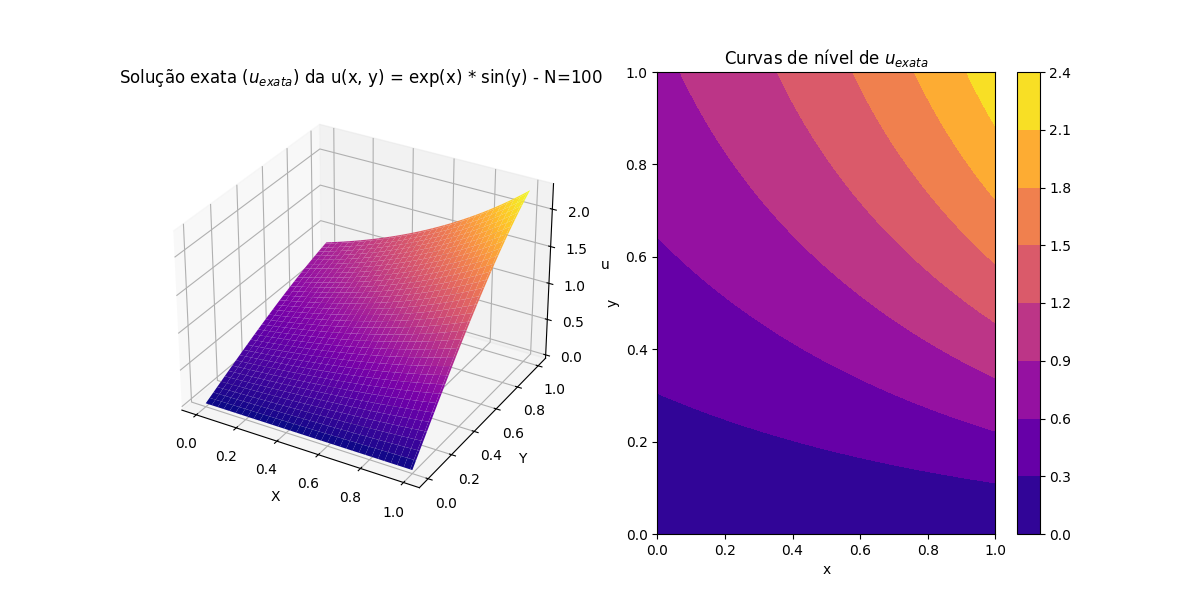
\includegraphics[width=\textwidth]{TAREFA_01/img/Problem1/b_100.png}
                        \caption{Simulação 1B com $N = 100$}
                    \end{minipage}
                \end{figure}
            \end{enumerate}

            \item Considere a equação de Poisson ($\Delta u = f$) no quadrado unitário $\Omega = (0, 1) \times (0, 1)$ com a função de força dada por:
            \begin{equation}
                f(x, y) = -2 \cos(x) \sin(y)
                \label{eq:enunciado-2a}
            \end{equation}

            Para resolver essa equação de Poisson, consideramos a solução exata:
            \begin{equation}
                u_{\text{exata}}(x,y) = \cos(x)\sin(y)
                \label{eq:enunciado-2b}
            \end{equation}

            Considerando condições de fronteira de Dirichlet dadas pela solução exata:
            \begin{enumerate}
                \item Verifique que a Equação \eqref{eq:enunciado-2b} satisfaz a equação com a função de força dada pela Equação \eqref{eq:enunciado-2a}

                Na resolução dessa questão, criamos uma função de verificação como segue: 

                \begin{lstlisting}
# Funcao para verificar se a equacao eh satisfeita
def verify() -> bool:
    # Definindo uma malha de pontos para x e y no intervalo [0, 1] com 5 divisoes
    X = np.linspace(0, 1, 5)
    Y = np.linspace(0, 1, 5)
    
    # Loop pelos valores de X e Y
    for x in X:  
        for y in Y:  
            left = f(x, y)  # esquerda da equacao, o valor de f(x, y)
            right = -2 * np.cos(x) * np.sin(y)  # direita da equacao

            # Verifica se a parte esquerda eh aproximadamente igual a direita
            if not np.isclose(left, right):
                # Se os valores nao forem proximos, imprime um erro com os valores correspondentes de x e y
                print(f"Erro: para (x={x}, y={y}), esquerda = {left}, direita = {right}")
                return False  # Retorna False para indicar que a equacao nao foi satisfeita
    
    return True  # A solucao u(x, y) satisfaz a equacao com a funcao f(x, y)
                \end{lstlisting}

    Validando o item (a) com sua função, teremos o seguinte retorno de código: 

\begin{lstlisting}
print("Validando o item (a)")
verify()
# -> True
\end{lstlisting}
                
                \item Realize simulações para valores de $N = 50, 100, 200$ e plote as soluções numéricas e a solução exata.
                    
                    \textbf{Solução:}

                    \begin{figure}[H]
                    \centering
                    \begin{minipage}{0.32\textwidth}
                        \centering
                        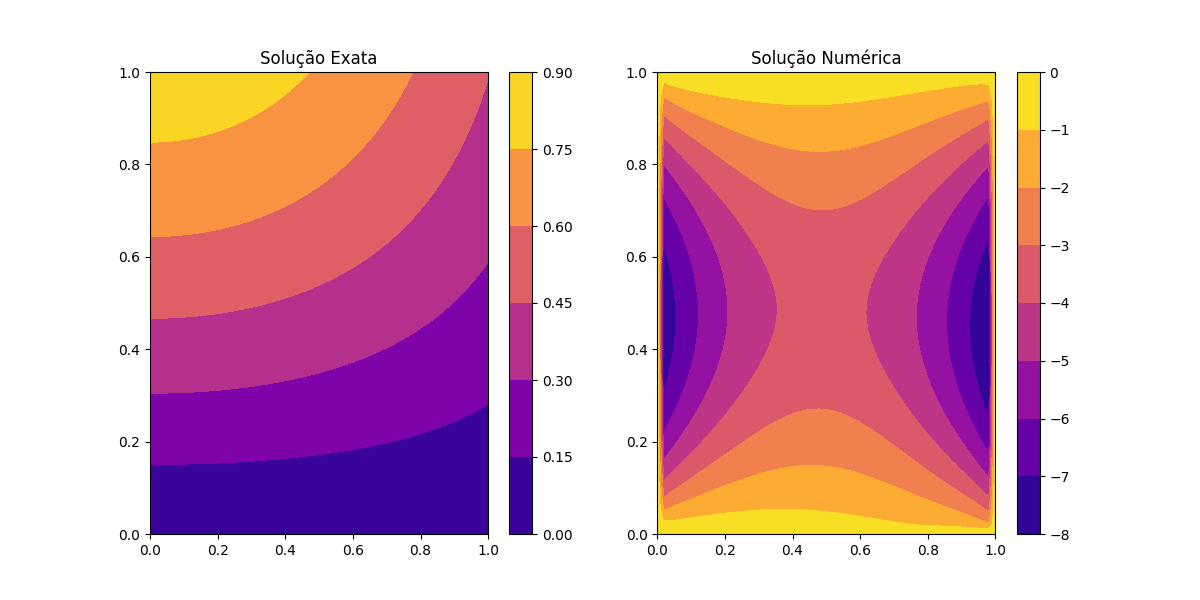
\includegraphics[width=\textwidth]{TAREFA_01/img/Problem2/50.png}
                        \caption{Simulação 2B com $N = 20$}
                    \end{minipage}
                    \hfill
                    \begin{minipage}{0.32\textwidth}
                        \centering
                        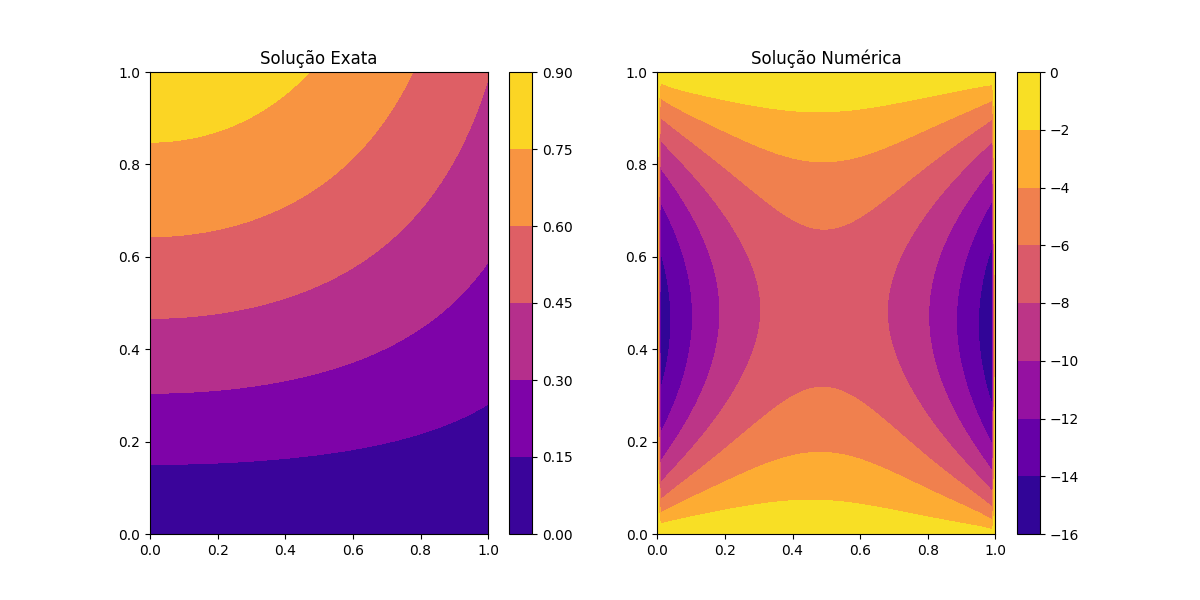
\includegraphics[width=\textwidth]{TAREFA_01/img/Problem2/100.png}
                        \caption{Simulação 2B com $N = 100$}
                    \end{minipage}
                    \hfill
                    \begin{minipage}{0.32\textwidth}
                        \centering
                        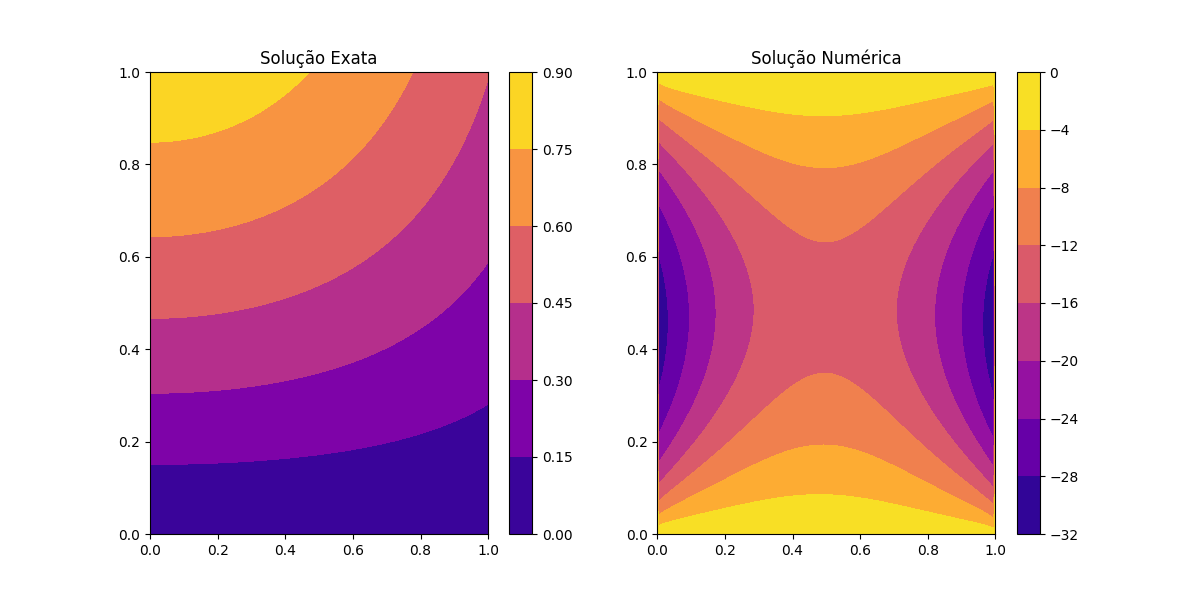
\includegraphics[width=\textwidth]{TAREFA_01/img/Problem2/200.png}
                        \caption{Simulação 2B com $N = 200$}
                    \end{minipage}
                \end{figure}
                
                \item Imprima os erros em relação à solução exata contínua.

                \textit{Observação: Para este relatório, apresentamos $20\%$ dos valores assumidos por $x$ e 4 valores de $y$ para tornar a apresentação mais clara. A tabela completa está disponível nos códigos e arquivos \textit{.csv} anexados.}

    
                \begin{table}[H]
                    \centering
                    \caption{Erro calculado na simulação $N=50$}
                    \label{tab:erro_xy_50}
                    \renewcommand{\arraystretch}{1.25}
                    \setlength{\tabcolsep}{12pt}
                    \begin{tabular}{|c|c|c|c|c|}
                        \hline
                        \textbf{$x$} & \textbf{$y = 0.00$} & \textbf{$y = 0.24$} & \textbf{$y = 0.47$} & \textbf{$y = 0.71$} \\ \hline
                        0.00 & 0.000000 & 0.000000 & 0.000000 & 0.000000 \\ \hline
                        0.10 & 0.099833 & 1.882937 & 1.616623 & 2.112684 \\ \hline
                        0.20 & 0.198669 & 3.290300 & 2.644325 & 3.354436 \\ \hline
                        0.29 & 0.295520 & 4.328647 & 3.445981 & 4.265023 \\ \hline
                        0.39 & 0.389418 & 4.958013 & 3.957576 & 4.799946 \\ \hline
                        0.49 & 0.479426 & 5.178478 & 4.148823 & 4.953132 \\ \hline
                        0.59 & 0.564642 & 5.004041 & 4.017148 & 4.737323 \\ \hline
                        0.69 & 0.644218 & 4.454460 & 3.582953 & 4.178380 \\ \hline
                        0.78 & 0.717356 & 3.555614 & 2.888192 & 3.317695 \\ \hline
                        0.88 & 0.783327 & 2.351951 & 1.997187 & 2.221227 \\ \hline
                    \end{tabular}
                \end{table}
    
                \begin{table}[H]
                    \centering
                    \caption{Erro calculado na simulação $N=100$}
                    \label{tab:erro_xy_100}
                    \renewcommand{\arraystretch}{1.25}
                    \setlength{\tabcolsep}{12pt}
                    \begin{tabular}{|c|c|c|c|c|}
                        \hline
                        \textbf{$x$} & \textbf{$y = 0.00$} & \textbf{$y = 0.25$} & \textbf{$y = 0.50$} & \textbf{$y = 0.74$} \\ \hline
                        0.00 & 0.000000 & 0.000000 & 0.000000 & 0.000000 \\ \hline
                        0.05 & 0.049979 & 1.800425 & 1.580714 & 2.211568 \\ \hline
                        0.10 & 0.099833 & 3.290075 & 2.649791 & 3.674547 \\ \hline
                        0.15 & 0.149438 & 4.663765 & 3.657335 & 5.017072 \\ \hline
                        0.20 & 0.198669 & 5.883958 & 4.577122 & 6.202277 \\ \hline
                        0.25 & 0.247404 & 6.927325 & 5.386953 & 7.208167 \\ \hline
                        0.30 & 0.295520 & 7.781173 & 6.069078 & 8.023337 \\ \hline
                        0.35 & 0.342898 & 8.439803 & 6.610197 & 8.643080 \\ \hline
                        0.40 & 0.389418 & 8.901834 & 7.001193 & 9.066735 \\ \hline
                        0.45 & 0.434966 & 9.168515 & 7.236726 & 9.296104 \\ \hline
                        0.50 & 0.479426 & 9.242750 & 7.314824 & 9.334585 \\ \hline
                        0.54 & 0.522687 & 9.128568 & 7.236536 & 9.186741 \\ \hline
                        0.59 & 0.564642 & 8.830868 & 7.005679 & 8.858139 \\ \hline
                        0.64 & 0.605186 & 8.355364 & 6.628709 & 8.355390 \\ \hline
                        0.69 & 0.644218 & 7.708736 & 6.114688 & 7.686390 \\ \hline
                        0.74 & 0.681639 & 6.899043 & 5.475334 & 6.860820 \\ \hline
                        0.79 & 0.717356 & 5.936584 & 4.725096 & 5.891004 \\ \hline
                        0.84 & 0.751280 & 4.835443 & 3.881186 & 4.793198 \\ \hline
                        0.89 & 0.783327 & 3.615889 & 2.963487 & 3.589201 \\ \hline
                        0.94 & 0.813416 & 2.307188 & 1.994244 & 2.307665 \\ \hline
                    \end{tabular}
                \end{table}
    
    
                \begin{table}[H]
                    \centering
                    \caption{Erro calculado na simulação $N=200$}
                    \label{tab:erro_xy_200}
                    \renewcommand{\arraystretch}{1.25}
                    \setlength{\tabcolsep}{12pt}
                    \begin{tabular}{|c|c|c|c|c|}
                        \hline
                        \textbf{$x$} & \textbf{$y = 0.00$} & \textbf{$y = 0.25$} & \textbf{$y = 0.50$} & \textbf{$y = 0.75$} \\ \hline
                        0.00 & 0.000000 & 0.000000 & 0.000000 & 0.000000 \\ \hline
                        0.02 & 0.019999 & 1.461875 & 1.337067 & 1.886796 \\ \hline
                        0.04 & 0.039989 & 2.667926 & 2.190556 & 3.083192 \\ \hline
                        0.06 & 0.059964 & 3.857494 & 3.035968 & 4.262617 \\ \hline
                        0.08 & 0.079915 & 5.023001 & 3.869449 & 5.417385 \\ \hline
                        0.10 & 0.099833 & 6.157533 & 4.687248 & 6.540515 \\ \hline
                        0.12 & 0.119712 & 7.254949 & 5.485749 & 7.625847 \\ \hline
                        0.14 & 0.139543 & 8.309931 & 6.261493 & 8.668087 \\ \hline
                        0.16 & 0.159318 & 9.317985 & 7.011203 & 9.662789 \\ \hline
                        0.18 & 0.179030 & 10.275386 & 7.731804 & 10.606301 \\ \hline
                        0.20 & 0.198669 & 11.179117 & 8.420429 & 11.495686 \\ \hline
                        0.22 & 0.218230 & 12.026776 & 9.074439 & 12.328629 \\ \hline
                        0.24 & 0.237703 & 12.816498 & 9.691418 & 13.103346 \\ \hline
                        0.26 & 0.257081 & 13.546865 & 10.269181 & 13.818498 \\ \hline
                        0.28 & 0.276356 & 14.216838 & 10.805773 & 14.473115 \\ \hline
                        0.30 & 0.295520 & 14.825685 & 11.299460 & 15.066528 \\ \hline
                        0.32 & 0.314567 & 15.372932 & 11.748732 & 15.598318 \\ \hline
                        0.34 & 0.333487 & 15.858310 & 12.152287 & 16.068264 \\ \hline
                        0.36 & 0.352274 & 16.281724 & 12.509030 & 16.476315 \\ \hline
                        0.38 & 0.370920 & 16.643219 & 12.818060 & 16.822552 \\ \hline
                        0.40 & 0.389418 & 16.942954 & 13.078665 & 17.107171 \\ \hline
                        0.42 & 0.407760 & 17.181186 & 13.290309 & 17.330460 \\ \hline
                        0.44 & 0.425939 & 17.358254 & 13.452628 & 17.492789 \\ \hline
                        0.46 & 0.443948 & 17.474564 & 13.565421 & 17.594595 \\ \hline
                        0.48 & 0.461779 & 17.530584 & 13.628641 & 17.636378 \\ \hline
                        0.50 & 0.479426 & 17.526836 & 13.642390 & 17.618691 \\ \hline
                        0.52 & 0.496880 & 17.463888 & 13.606916 & 17.542140 \\ \hline
                        0.54 & 0.514136 & 17.342356 & 13.522605 & 17.407378 \\ \hline
                        0.56 & 0.531186 & 17.162898 & 13.389980 & 17.215108 \\ \hline
                        0.58 & 0.548024 & 16.926217 & 13.209698 & 16.966079 \\ \hline
                        0.60 & 0.564642 & 16.633058 & 12.982549 & 16.661093 \\ \hline
                        0.62 & 0.581035 & 16.284216 & 12.709451 & 16.301004 \\ \hline
                        0.64 & 0.597195 & 15.880535 & 12.391458 & 15.886728 \\ \hline
                        0.66 & 0.613117 & 15.422918 & 12.029754 & 15.419245 \\ \hline
                        0.68 & 0.628793 & 14.912336 & 11.625655 & 14.899616 \\ \hline
                        0.70 & 0.644218 & 14.349838 & 11.180616 & 14.328987 \\ \hline
                        0.72 & 0.659385 & 13.736566 & 10.696224 & 13.708612 \\ \hline
                        0.74 & 0.674288 & 13.073777 & 10.174208 & 13.039867 \\ \hline
                        0.76 & 0.688921 & 12.362868 & 9.616434 & 12.324278 \\ \hline
                        0.78 & 0.703279 & 11.605403 & 9.024911 & 11.563548 \\ \hline
                        0.80 & 0.717356 & 10.803155 & 8.401786 & 10.759585 \\ \hline
                        0.82 & 0.731146 & 9.958146 & 7.749346 & 9.914547 \\ \hline
                        0.84 & 0.744643 & 9.072699 & 7.070015 & 9.030875 \\ \hline
                        0.86 & 0.757843 & 8.149492 & 6.366347 & 8.111341 \\ \hline
                        0.88 & 0.770739 & 7.191612 & 5.641024 & 7.159079 \\ \hline
                        0.90 & 0.783327 & 6.202604 & 4.896841 & 6.177620 \\ \hline
                        0.92 & 0.795602 & 5.186507 & 4.136700 & 5.170910 \\ \hline
                        0.94 & 0.807558 & 4.147869 & 3.363597 & 4.143303 \\ \hline
                        0.96 & 0.819192 & 3.091718 & 2.580601 & 3.099536 \\ \hline
                        0.98 & 0.830497 & 2.023504 & 1.790843 & 2.044666 \\ \hline
                    \end{tabular}
                \end{table}
            \end{enumerate}
        \end{enumerate}

    \section{Conclusão}

        Neste trabalho, exploramos a solução numérica da equação de Poisson utilizando o método de diferenças finitas em um domínio unitário, sob condições de contorno de Dirichlet. A implementação foi bem-sucedida em gerar soluções numéricas para diferentes valores de $N$, e conseguimos observar a convergência do erro à medida que o espaçamento da malha diminuía.
        
        A análise das tabelas de erro revelou que, para valores maiores de $N$, o erro absoluto calculado em pontos do domínio diminui significativamente, confirmando a eficiência do método. Por exemplo, quando $N = 20$, o erro era mais perceptível, especialmente nas regiões próximas às bordas do domínio. No entanto, ao aumentar $N$ para $50$ e $100$, o erro diminuiu consideravelmente, provando a consistência do método e a tendência de convergência da solução numérica para a solução exata conforme a malha se tornava mais refinada.
        
         Ao longo do processo, identificamos aspectos importantes relacionados à estimação do erro e à consistência do método. Um ponto que se destacou foi a importância de definir corretamente as condições de contorno, que têm um impacto direto nos resultados obtidos.
        
        Em resumo, este estudo proporcionou um entendimento mais profundo sobre a aplicação de métodos numéricos a equações diferenciais, mostrando a eficácia do método de diferenças finitas e a relevância da análise de erro para validar as soluções numéricas.
        
    
    \renewcommand{\bibsection}{}
    
    \section{Referências}
        \nocite{*}
        \bibliographystyle{abbrv}
        \bibliography{referencias}
        
\end{document}